% Sample document for SBGames papers
% Uses a slightly modified IEEE VGTC template in conference mode

\documentclass{vgtc}                          % final (conference style)

%% These three lines bring in essential packages: ``mathptmx'' for Type 1 
%% typefaces, ``graphicx'' for inclusion of EPS figures. and ``times''
%% for proper handling of the times font family.

\usepackage{mathptmx}
\usepackage{graphicx}
\usepackage{times}
\usepackage[brazil,american]{babel}
\usepackage[utf8]{inputenc}
\usepackage{hyperref}


%% We encourage the use of mathptmx for consistent usage of times font
%% throughout the proceedings. However, if you encounter conflicts
%% with other math-related packages, you may want to disable it.

%% If you are submitting a paper to a conference for review with a double
%% blind reviewing process, please replace the value ``0'' below with your
%% OnlineID. Otherwise, you may safely leave it at ``0''.
\onlineid{0}

%% declare the category of your paper, only shown in review mode
\vgtccategory{Research}

%% Paper title.

\title{Projeto prático usando o microprocessador MIPS no kit de desenvolvimento DE2-70.}

%% Authors are listed in up to three columns as necessary
%% with a footnote referring to a single e-mail contact.
%% Affiliations are placed after the authors, one per line
%% with superscript numbers used to link them to authors

%% Single author:
%%\author{Single author name\thanks{e-mail: email@somewhere.com}}
%%\affiliation{\scriptsize University A}

%% Multiple authors with single affiliation:
%%\author{First author\thanks{e-mail: email@somewhere.com} %
%%\and Second author %
%%\and Third author}
%%\affiliation{\scriptsize Research institute X}

%% Multiple authors with multiple affiliations:

	
\author{Dayanne Fernandes da Cunha, 13/0107191$^{1}$ \thanks{e-mail: dayannefernandesc@gmail.com}%
\and Diego Vaz Fernandes, 16/0117925$^{1}$\thanks{e-mail: diego.vazfernandes@hotmail.com}%
\and Lucas Junior Ribas, 16/0052289$^{1}$\thanks{e-mail: ribas858@gmail.com@gmail.com}
\and Lucas Mafra Chagas, 12/0126443$^{1}$\thanks{e-mail: chagas.lucas.mafra@gmail.com}
\and Marcelo Giordano Martins Costa de Oliveira, 12/0037301$^{1}$\thanks{e-mail: marcelo.giordano@gmail.com}}
\affiliation{\scriptsize $^{1}$Universidade de Brasília, Departamento de Ciência da Computação, Brasil}

%% A teaser figure can be included as follows:
\teaser{
  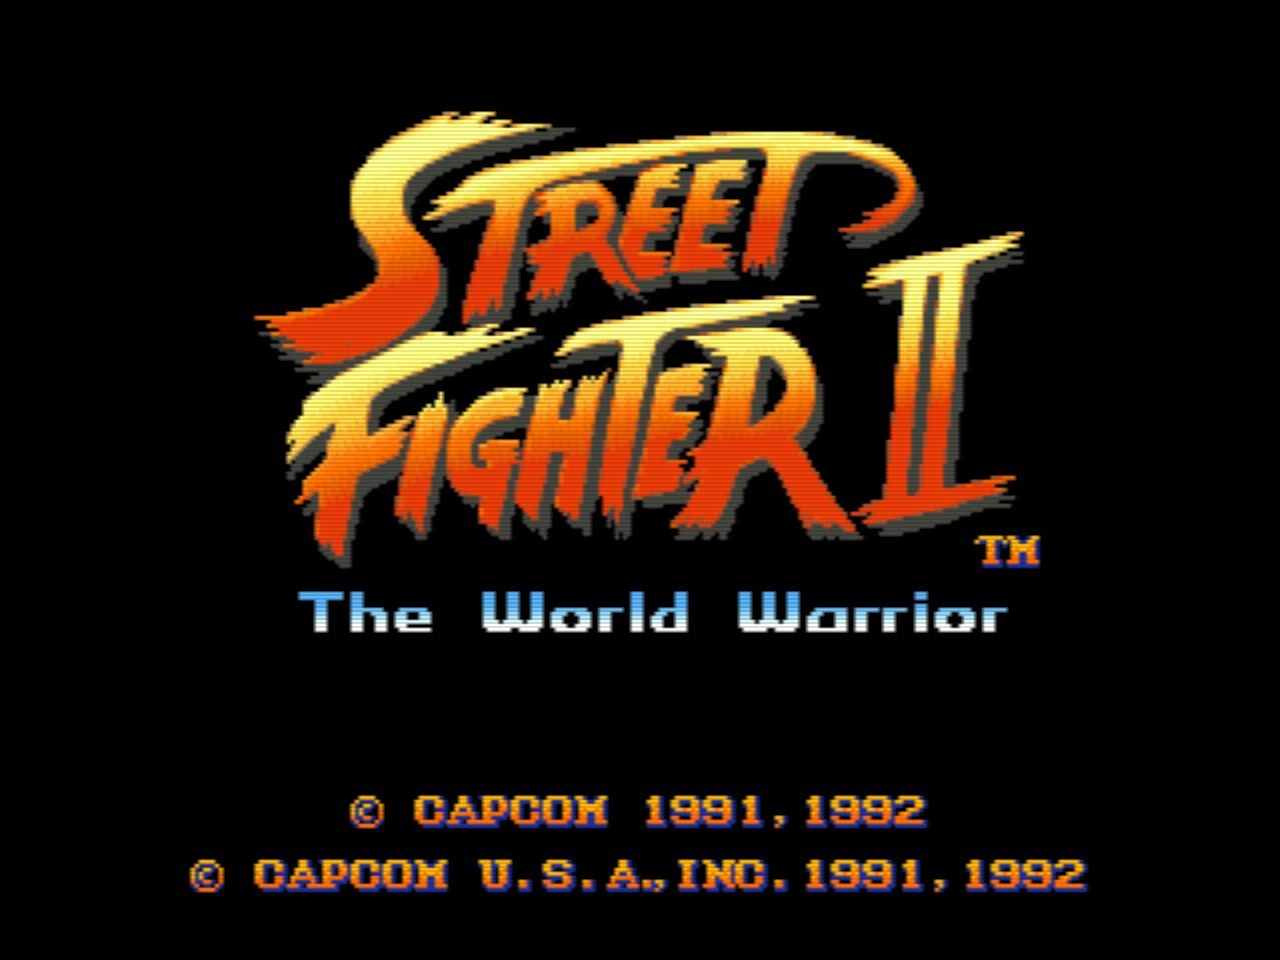
\includegraphics[width=2in]{street-fighter.jpg}
  \caption{Projeto prático Street Figther 2.}
}

%% Abstract section.
%% Note how the keywords must be also included in this section!
\abstract{ The main goal of this project is to build the game Street Fighter 2 using microprocessor MIPS on development kit DE2-70, apllying the content learning during the course. 

\smallskip

\noindent \textbf{Keywords:} Street Fighter 2, Microprocessador MIPS, MIPS Pipeline, DE2-70, Cartão SD.
} % end of abstract

%% Copyright space is enabled by default as required by guidelines.
%% It is disabled by the 'review' option or via the following command:
% \nocopyrightspace

%%%%%%%%%%%%%%%%%%%%%%%%%%%%%%%%%%%%%%%%%%%%%%%%%%%%%%%%%%%%%%%%
%%%%%%%%%%%%%%%%%%%%%% START OF THE PAPER %%%%%%%%%%%%%%%%%%%%%%
%%%%%%%%%%%%%%%%%%%%%%%%%%%%%%%%%%%%%%%%%%%%%%%%%%%%%%%%%%%%%%%%%

\begin{document}

%% The ``\maketitle'' command must be the first command after the
%% ``\begin{document}'' command. It prepares and prints the title block.

%% the only exception to this rule is the \firstsection command
\firstsection{Introdução}

\maketitle

%% do not uncomment this; use the \firstsection above
%%\section{Introduction} 

Como forma de avaliação na matéria Organização e Arquitetura de Computadores, o Professor Dr. Marcus Vinicius Lamar propós aos seus alunos o desenvolvimento do jogo mundialmente conhecido Street Fighter 2. Street Fighter 2 é um jogo de luta 2D criado em 1991 pela empresa japonesa Capcom.

Para o desenvolvimento do projeto, os alunos precisariam cumprir alguns critérios para conseguir a nota máxima. Eles foram divididos em duas categorias, Requerimentos de Hardware e Requerimentos de Software. Para os Requerimentos de Hardware, os estudantes precisavam usar o processador MIPS Pipeline, apresentar o uso adequado do teclado, apresentar efeitos sonoros e música, além de usar o cartão SD para o armazenamento de dados.

Quanto aos Requerimentos de Software, o grupo precisava implementar um jogo plenamente funcional, com menu, apresentação e todos os outros detalhes que o jogo possui. A equipe precisava apresentar dois modos de jogo: Arcade, onde o jogador joga contra o computador escolhendo o seu nível e evoluindo de fase, e Versus, onde há a presença de dois jogadores, ambos com três rounds. Além disso, era preciso mostrar os doze personagens presentes dentro do jogo, com suas respectivas arenas e golpes especiais. 


\section{Fundamentação Teórica e Técnica}

Para cumprir os Requerimentos de Hardware, as equipes precisavam ter o conhecimento sobre MIPS Pipeline, funcionamento da interface do teclado ps2, interface VGA e interface de audio CODEC.

Como explicitado no livro Organização e Projeto de Computadores, dos autores David A. Patterson e John LeRoy Hennessy, Pipelining é uma técnica de implementação em que várias instruções são sobrepostas na execução, sendo fundamental para tornar os processadores mais rápidos atualmente. 

\begin{figure}[htb]
  \centering
  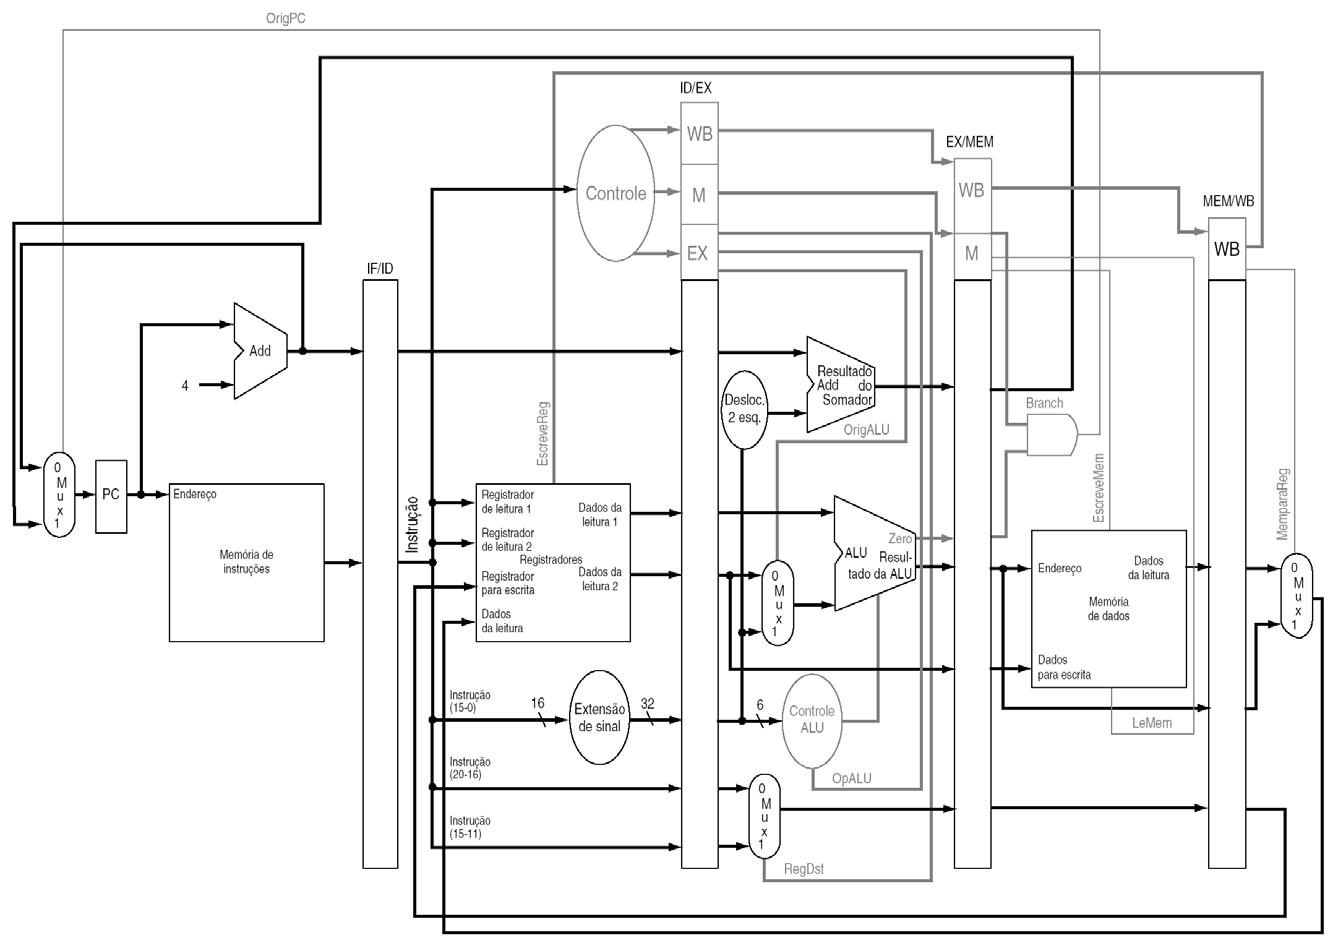
\includegraphics[width=2.76in]{pipeline.jpg}
 \caption{Caminho de Dados Pipeline}
\end{figure}

 
Com esse conhecimento em mente, onde várias instruções são sobrepostas na execução, é necessário tratar os riscos presentes de modo com que não perca sua eficiência. Para isso, é importante entender os Hazards, responsáveis por prevenir com que a próxima instrução da fila seja executado em determinado ciclo de clock. Existem três tipos de Hazards, os Hazards Estruturais, os Hazards de Dados e os Hazards de Controle.

Os Hazards Estruturais acontecem quando o hardware não admite a combinação de instruções em um mesmo ciclo de clock ou a unidade funcional está ocupada no momento. Os Hazards de Dados acontecem quando o pipeline precisa ser interrompido porque uma etapa ainda precisa esperar até que a outra seja concluida. Já o Hazard de Controle tem a necessidade de tomar uma decisão com base nos resultados de uma instrução enquanto outras estão sendo executadas.

Para solucionar esses Hazards o desenvolvedor pode inserir bolhas entre as instruções, executar as instruções fora de ordem ou dando forwarding.

Ao passar as instruções para a placa DE2-70, é necessário entender o seu funcionamento, sabendo suas entradas, os interruptores e botões.


\begin{figure}[htb]
  \centering
  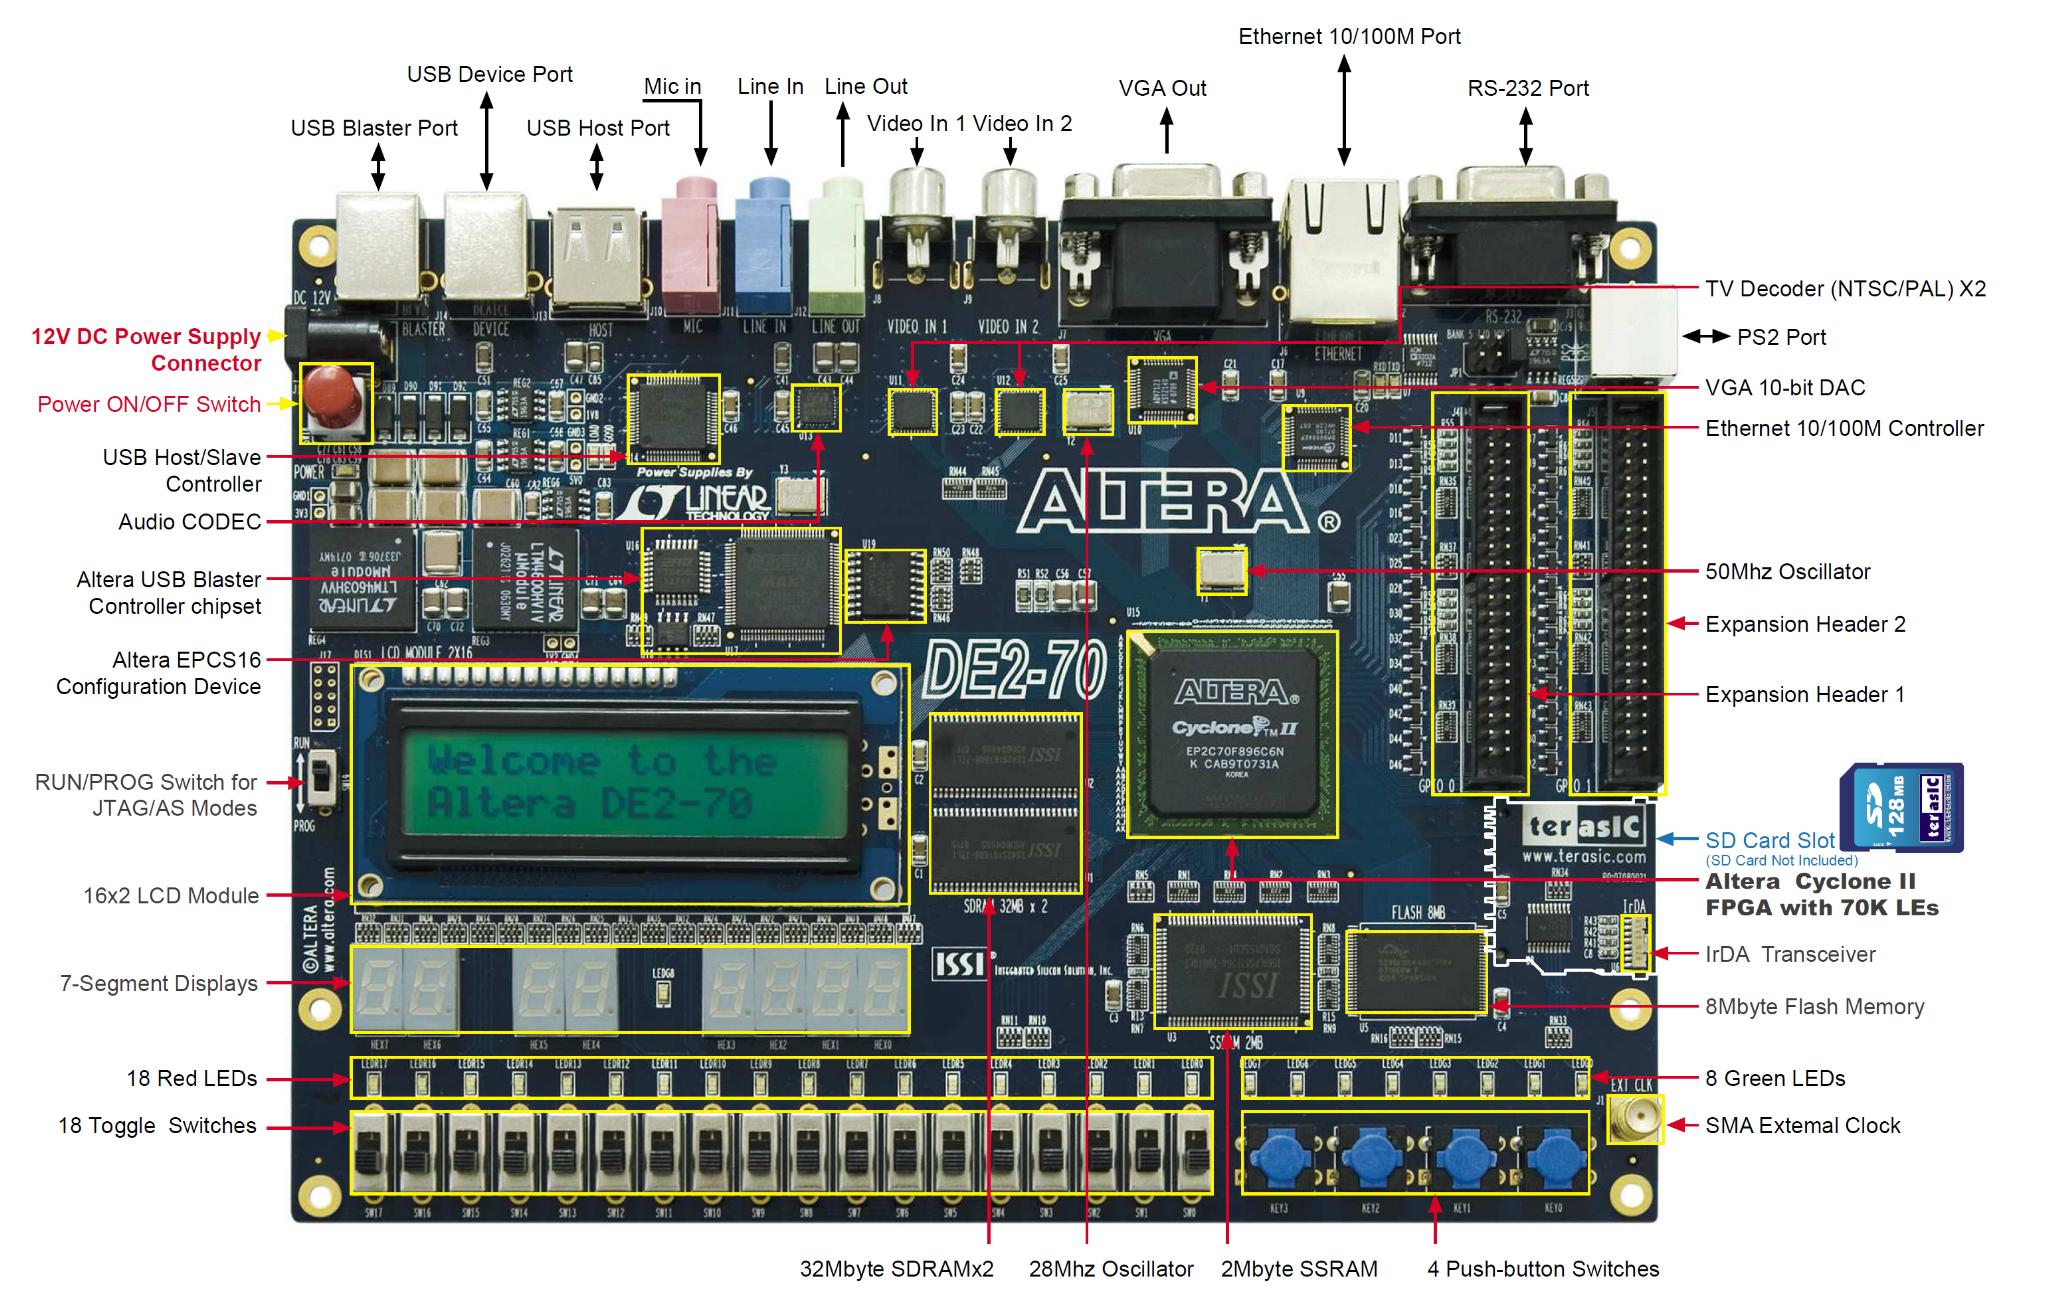
\includegraphics[width=2.76in]{altera.jpg}
 \caption{Mapa de utilização da DE2-70}
\end{figure}


As interfaces utilizadas para o desenvolvimento do projeto são: VGA, Teclado PS2, Sintetizador de áudio polifônico e Cartão SD. Foi disponibilizado um arquivo contendo uma explicação sobre cada interface, mostrando seu funcionamento e exemplos de uso.


A interface do VGA carrega o arquivo $.mif$ em sua memória inicializar o processador, sendo as dimensões necessárias 320x240 pixels.

A interface do cartão SD funciona por MMIO, onde seis bytes de memória são endereçados para o controlador do cartão SD, sendo eles:
\begin{itemize}
\item SDINTERFACEADDR: Recebe o endereço físico de memória do byte a ser lido do cartão SD. O endereço pode ser obtido lendo o cartão SD em um editor de memória em um computador.
\item SDINTERFACECTRL: Fornece ao software informações do estado do controlador. Caso o valor lido seja 0x00, o controlador se encontra em estado READY, significando que o byte da última leitura está pronto para ser obtido e que uma nova leitura já pode ser realizada. Caso o valor lido seja diferente de 0x00, o controlador estará em estado BUSY, significando que o último byte pedido ainda não está pronto ou o cartão ainda não inicializou. O valor de SDINTERFACECTRL em estado BUSY mostra qual o último comando enviado ao cartão SD e serve para depuração.
\item SDINTERFACEDATA: Fornece o byte lido do cartão.
\end{itemize}

O cartão SD possui o limite de no máximo 2GB de armazenamento, a implementação utiliza o modo SPI de comunicação e a frequência SCLK de inicialização é de 400 KHz e de 25 MHz para operações de leitura.

Nos endereços TecladoBuffer0 e TecladoBuffer1 está o buffer da interface do teclado PS2. O byte menos significativo de Buffer0 contém o código mais recente enviado, assim é possivel mapear o teclado e qual tecla foi clicada.
   
A interface do áudio utiliza uma memória de dados de duas portas UserData e BlockDouble. Uma porta de escrita e leitura para o uso da CPU e uma porta somente de leitura para o sintetizador. É utilizada na configuração do syscall 31 e syscall 33

Para cumprir os Requerimentos de Software, os grupos precisavam, atráves da escolha do microprocessador, desenvolver em MIPS Assembly todas as rotinas necessárias para o funcionamento do jogo.

Um processador MIPS consiste em uma unidade central processadora de inteiros e um conjunto de coprocessadores para tarefas auxiliares. O Coprocessador 0 gerencia traps, interrupções, exceções, memória cache e memória virtual. O Coprocessador 1 é a unidade processadora de números em ponto flutuante e os outros Coprocessadores são processadores de aplicações específicas.

\begin{figure}[htbp]
  \centering
  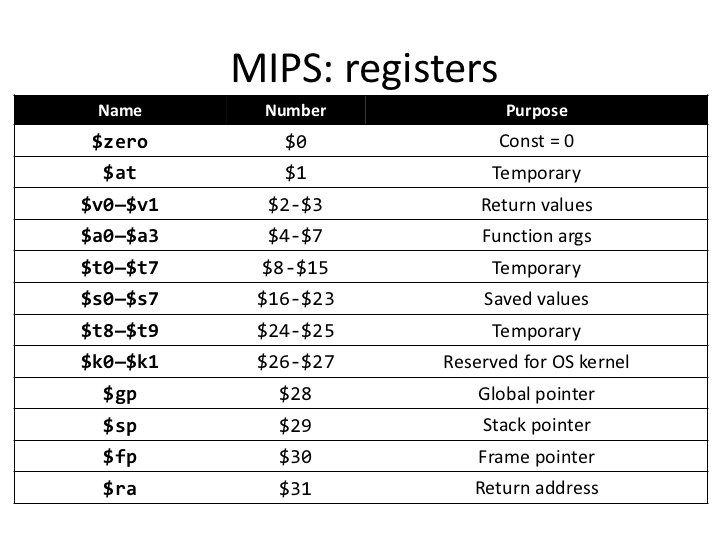
\includegraphics[width=2in]{register.jpg}
 \caption{Registradores MIPS Assembly}
\end{figure}

Todos os registradores são fisicamente iguais, com exceção do \$zero e \$ra. Portanto, a convenção é o uso sugerido para padronização

Já os princípios utilizados no projeto da ISA MIPS:
\begin{itemize}
\item Simplicidade favorece regularidade.
\item Menor significa mais rápido.
\item Bons projetos exigem bons compromissos. 
\end{itemize}



\begin{figure}[htbp]
  \centering
  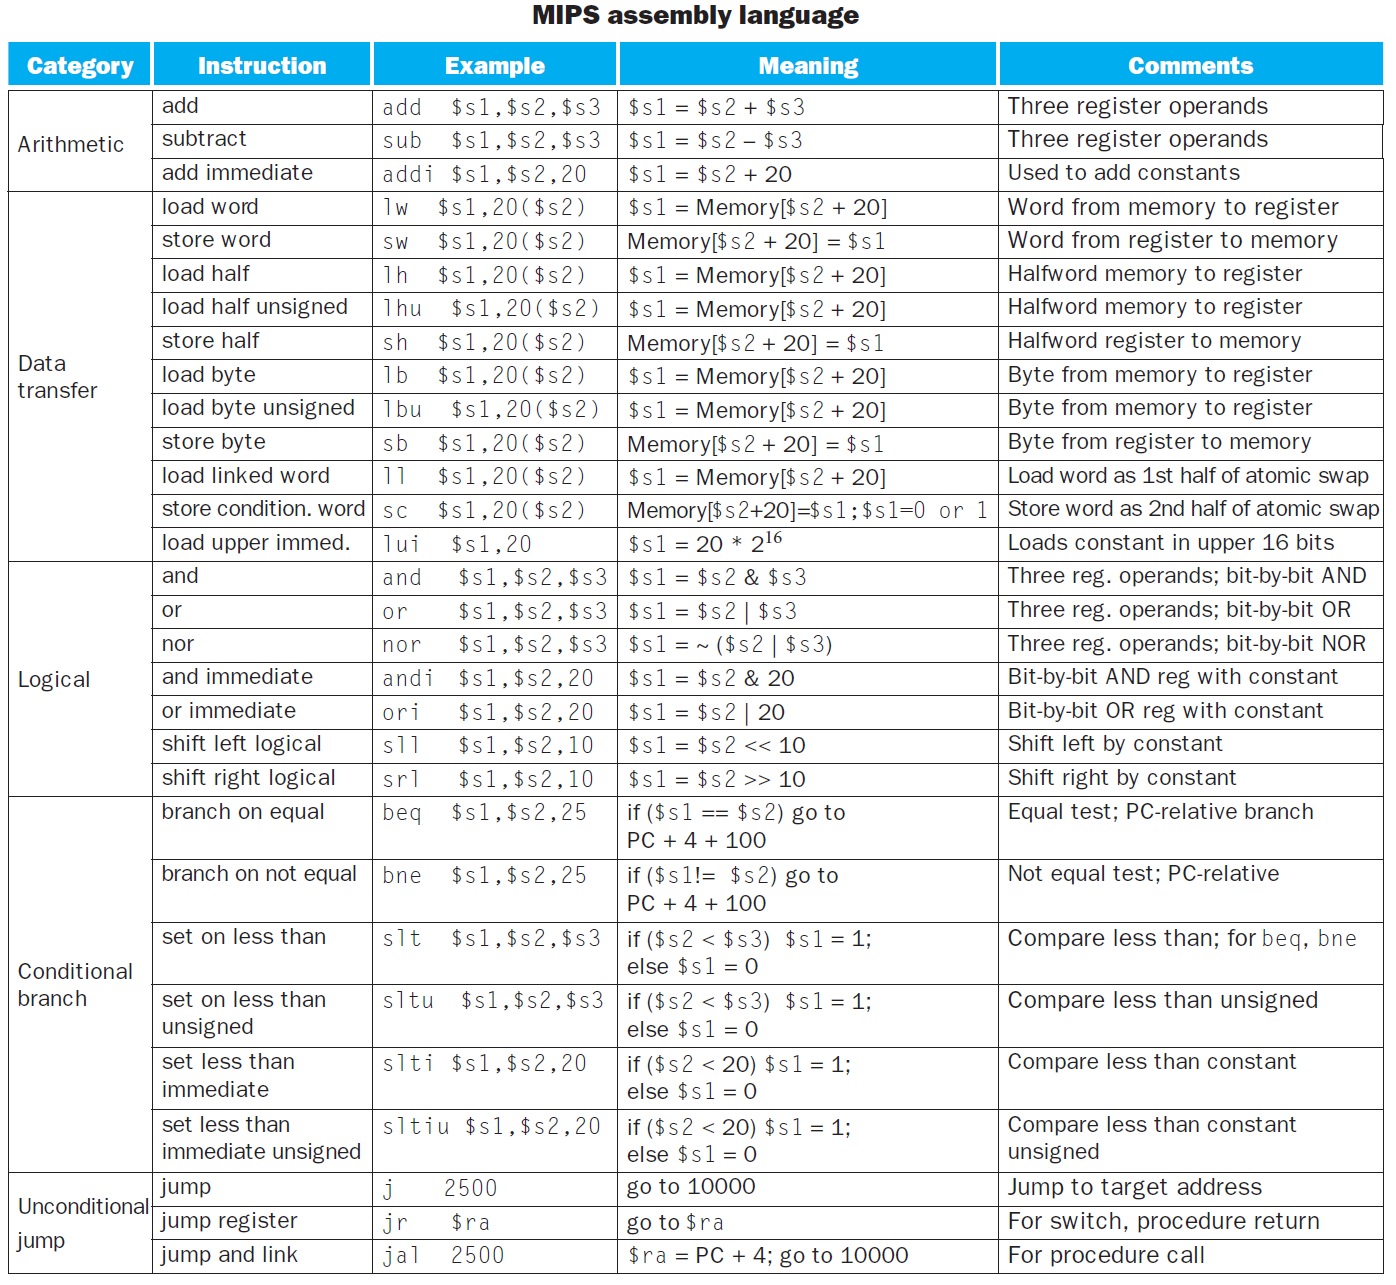
\includegraphics[width=2.76in]{assembly.png}
 \caption{Linguagem MIPS Assembly}
\end{figure}

As instruções pertencem a três tipos de formatos: Tipo-R, Tipo-I e Tipo-J. As instruções do Tipo-R são referentes a registradores do tipo de instrução. As instruções do Tipo-I são do tipo imediato e as do Tipo-J são referente a instruções de pulo.  


\section{Metodologia}

A parte lógica do jogo consiste em trabalhar com as sprites do jogo, fazendo uma integração entre os cenários, ícones e personagens.

As sprites presentes no jogo seguiram alguns padrões para que fosse possível a sua leitura e que não atrapalhasse na construção dos cenários. Todas as imagens precisavam ter 320pixels de largura e 240 pixels de altura para facilitar o mapeamento da VGA. 

Já as imagens que interagem com o cenário, como os personagens e ícones de seleção, apresentaram um fundo na cor 0xC7, que é considerado transparente para o MIPS da DE2-70 e para o Mars, mostrando assim a integração entre os cenários e os ícones do jogo.  

Para a disponibilização dos cenários e personagens no jogo, os arquivos foram convertidos para um arquivo $.txt$ , pois a DE2-70 trabalha reconhecendo os caracteres da tabela ASCII e a partir disso formar a imagem no display. Os arquivos foram alocados no cartao SD de forma sequencial para facilitar a leitura e tambem o nosso mapeamento da memoria do mesmo, o código escrito em assembly MIPS programa a placa para realizar a leitura do SD e os dados obtidos eram armazenados na SRAM da placa. 

Apesar da memória SRAM da placa ser muito escassa, a velocidade de acesso é muito superior a do SD e isso foi uma grande estratégia no momento de carregar as sprites, pois ao salva-las do SD para a SRAM, ela não precisaria ser lida novamente e assim sendo exibido com muito mais agilidade na VGA.  

O maior problema que tivemos foi o calculo do offset do SD, pois ele varia de cartao para cartao e fatores como fabricação, tamanho influenciavam na defasagem do cartão. Ao descobrimos o valor em hexadecimal da defasagem do SD somavamos esse valor ao endereco inicial de onde estavam os cenários que queriamos ler, após a soma desse valor a leitura dos pixels salvos na SRAM eram lidos de forma correta e escritos na memoria VGA, exibindo a imagem perfeitamente na tela.

Com essa base fomos capazes de dar continuidade ao projeto, usando essas técnicas para armazenar os dados do game e poder carrega-los a qualquer momento, alternando quando conveniente de uma memória rápida para uma mais lenta e vice-versa.

Para a execução de áudio no jogo, editamos um arquivo $.midi$ para tocar sequencialmente na placa DE2-70, com os valores relacionados a cada nota tocada no nosso $user_data.mif$. Com base nas evoluções construídas por outros semestres referente a áudio, a interação entre áudio foi feita no syscall. Assim como nas imagens, os arquivos $.midi$ foram convertidos para $.txt$ para que fosse possível tocar as notas musicais de forma que a música original do jogo ficasse melhor representada.

Foi trabalhado com as seguintes variáveis da música: Quantidade de notas(QTDNOTAS), Delay entre notas(DELAY), Duração das Notas(DURACAO) e Valor das notas(NOTAS).As variáveis necessárias pelo syscall VOLUME e INSTRUMENTO não são representadas corretamente na placa, portanto foi mantido um valor padrão para que não fosse necessário alterar o código. Para a execução do áudio, foi utilizado a lógica de tocar UMA nota a cada loop da função main do código, e quando a música termina, volta para a primeira nota. 

Infelizmente não é a implementação ideal para um jogo atual, já que a música não é executada ao mesmo tempo de um clique no teclado, mas é o necessário para a implementação apresentada, visto que o jogo roda extremamente rápido no processador MIPS Pipeline. 

Os arquivos $.txt$ de áudio não foram armazenados no cartão SD, e sim na parte de memória de dados do usuário, por observar que a leitura dos $.txt$ dentro do cartão SD poderia demorar para ser lido e escrito no Buffer, resultando em uma demora de resposta entre a ação na tela e o áudio reproduzido.





\section{Resultados Obtidos}

Foi possível observar os resultados atráves do fluxo de tela a seguir:

Ao carregar o user code e o system code na DE2-70, depois de carregar as sprites do cartão SD, é apresentado a Tela Inicial.

Ao clicar no Enter, é apresentado o menu do jogo, onde o jogador pode escolher entre o modo Arcade ou o modo Versus.

Ao escolher o modo, o jogo é redirecionado para a escolha do personagem.

Após a escolha do personagem, o jogo é redirecionado para o mapa do jogador. No caso do Arcade, ele enfrenta um dos vilões do jogo. No caso do Versus, os jogadores se enfrentam no mapa do jogador 1.

\href{https://youtu.be/0BtsrIDkxic}{Demonstração do Jogo pt1.}
\href{https://youtu.be/fexJ_3Ww0OI}{Demonstração do Jogo pt2.}


\begin{figure}[htbp]
  \centering
  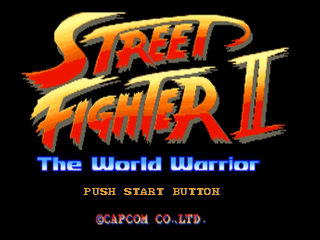
\includegraphics[width=2.5in]{abertura.png}
 \caption{Tela inicial.}
\end{figure}

\begin{figure}[htbp]
  \centering
  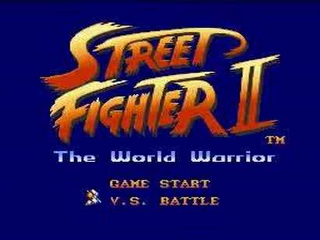
\includegraphics[width=2.5in]{versus.png}
 \caption{Menu principal.}
\end{figure}

\begin{figure}[htbp]
  \centering
  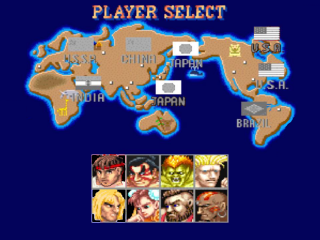
\includegraphics[width=2.5in]{select_vs.png}
 \caption{Menu de escolha de personagem.}
\end{figure}

\begin{figure}[htbp]
  \centering
  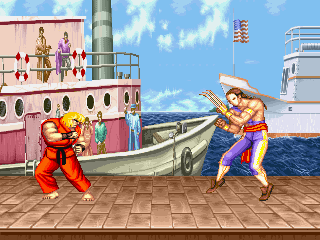
\includegraphics[width=2.5in]{ken_battle.png}
 \caption{Cenário com personagens.}
\end{figure}




%É possível ver os resultados no vídeo do youtube: \href{}{Demonstração do Jogo na Placa DE2-70}

\section{Conclusão}

O jogo foi desenvolvido integralmente na placa DE2-70, entretanto, não apresenta todas as funcionalidades pedidas nos Requisitos de Software, como um jogo plenamente funcional. Após a execução do projeto prático, foi possível observar o conteúdo apresentado durante o semestre. Foram observados os fundamentos teóricos e técnicos adquiridos durante os laboratórios e aulas em geral.

\section{Trabalhos Futuros}

Para trabalhos futuros, é possível observar os seguintes adendos que agregam o trabalho.


\begin{itemize}
\item Utilização da FPULA para uma melhor precisão na movimentação.
\item Adicionar outros modos de jogo.
\item Otimização do carregamento das sprites.
\item Adição de mais efeitos sonoros.
\item Inteligência artificial para os personagens no modo Arcade. 
\end{itemize} 


\section{Referência Bibliográfica}

\begin{itemize}
\item PATTERSON, David A.; HENNESY, John. Computer Organization and Design. 5. ed. [S.l.]: David A. Patterson And John LeRoy Hennesy, 2014. 856 p.
\item PRABHU, Gurpur M. . Pipeline Hazards. Disponível em: <http://web.cs.iastate.edu/~prabhu/Tutorial/PIPELINE/hazards.html>. Acesso em: 06 dez. 2017.
\item LAMAR, Marcus Vinicius . MAPA DE UTILIZAÇÃO DA DE2-70. Departamento de Ciência da Computação: [s.n.], 2017. 15 p.
\end{itemize}


\bibliographystyle{abbrv}
\bibliography{template}


\end{document}
